\begin{abstract}

TODO: rework abstract\\

Gridcoin [6] is a decentralized, open source math-based cryptocurrency which performs transactions without the need for a central issuing authority. Gridcoin securely rewards volunteer distributed computing performed upon the BOINC [5] platform in a decentralized manner. Available projects in BOINC in 2017 range from attempting to cure diseases like cancer [11,12,13], ebola [11], AIDS [11] and virus Zika [11], through orbit analysis and reconstruction of asteroids [14], through simulating earth in different ages to assess climate change [15], through mathematical research [16,17], through identification of subatomic particles [18] to scanning the sky for gravitational waves [19] and extraterrestrial intelligence [20].\\

Gridcoin is heavily based on Bitcoin [1] with the outstanding exception that Proof of Work where energy is wasted in inverting a hash function is replaced with the novel approach of Proof of Stake [2] linked to Distributed Proof of Research [3], developed on purpose for Gridcoin. The voting mechanism embedded in the blockchain which allows to choose which scientific projects to include in Proof of Research is outlined. In conclusion, an outlook is given on how Gridcoin could complement the way science is funded, sparking competition between traditionally funded science and gridcoin funded science.

\begin{center}
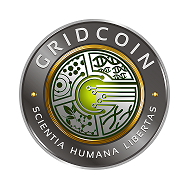
\includegraphics{figures/gridcoin-art-small}
\end{center}

\end{abstract}
